\section{Tutorial -- BSS-ANOVA}
\label{(sec.surrogate.bssanova)}

This tutorial covers the BSS-ANOVA surrogate modeling method.  The Bayesian
Smoothing Spline ANOVA (BSS-ANOVA) is essentially a Bayesian version of
ACOSSO \citep{Reich_2009}.  It is Gaussian Process (GP) model with a
non-conventional covariance function that borrows its form from SS-ANOVA.
It tackles the high dimensionality (of inputs) on two fronts: (1) variable
selection to eliminate uninformative variables from the model and (2)
restricting the level of interactions involved among the variables in the
model. This is done through a fully Bayesian approach which can also allow
for categorical input variables with relative ease. Since it is closely
related to ACOSSO, it generally works well in similar settings as
ACOSSO. The BSS-ANOVA procedure also allows for categorical inputs
\citep{Storlie_2013}. In this current implementation, BSS-ANOVA is more
computationally intensive than ACOSSO, so ACOSSO is preferred for faster
surrogate generation. 

This tutorial uses the same flowsheet and sample setup as the ALAMO
tutorial in Section \ref{sec.surrogate.alamo}. The statistics software
``R'' is also required to use ACOSSO and BSS-ANOVA. Before starting this
tutorial, you will need to install R version 3.1 or later (see \href{https://cran.r-project.org/}{\textcolor{blue}{http://cran.r-project.org/}}).

\begin{enumerate}
	\item{Set the path to the RScript executable.}
		\begin{enumerate}
			\item Click the \bu{Settings} button from the Home window.
			\item Change the RScript path if necessary.  The \bu{Browse} button opens a file browser that can be used to set the path.
		\end{enumerate}
	\item Complete the ALAMO tutorial in Section \ref{sec.surrogate.alamo} through Step 32, or load the FOQUS session saved after completing the ALAMO tutorial.
	\item Click the \bu{Surrogates} button from the Home window (Figure \ref{fig.bssanova.settings}).
	\item Select ``BSS-ANOVA'' in the \bu{Tool} drop-down list.
	\item Select the \bu{Method Settings} tab.
	\item Set ``Data Filter'' to ``Initial.''
	\item Set ``Use Flowsheet Data'' to ``Yes.''
	\item Set ``FOQUS Model (for UQ)'' to ``bssanova\_tutorial\_uq.py.''
	\item Set ``FOQUS Model (for Flowsheet)'' to ``bssanova\_tutorial\_fs.py.''
	\item Click the \bu{Run} icon (Figure \ref{fig.bssanova.settings}).
\end{enumerate}

\begin{figure}[H]
	\begin{center}
		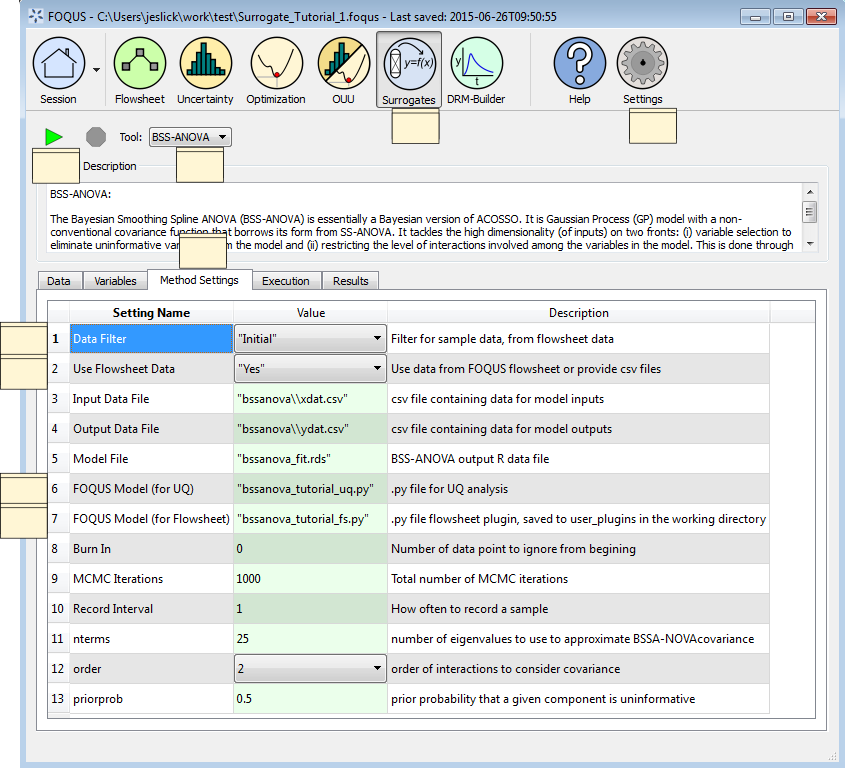
\includegraphics[scale=0.55]{Chapt_surrogates/figs/bssanova_settings}
		\caption{BSS-ANOVA Session Set Up}
		\label{fig.bssanova.settings}
	\end{center}
\end{figure}

\begin{enumerate}
   \setcounter{enumi}{10}
   \item The execution window will automatically display. While BSS-ANOVA is
     running, the execution window may show warnings, but this is normal.
   \item When the run completes, a UQ driver file is created, allowing the
     BSS-ANOVA surrogate to be used as a user-defined response surface in UQ
     analyses. (See Section \ref{tutorial.surrogate.uq}.)
   \item BSS-ANOVA also produces a flowsheet plugin.
\end{enumerate}

